\section{The pair background envelopes}
\label{sec:Envelopes}
For all ILC250 parameter sets, listed in Table~\ref{tab:Parameters}, a full bunch train (1312 bunch crossings) of the pair background particles were generated.
The \guineapig generation does not take the crossing angle of \SI{14}{\milli\radian} into account.
The calculation of the helix tracks that the pairs form in the SiD solenoid field with a strength of \SI{5}{\tesla} was done using the algorithm descibed in a former note presenting the pair envelopes of the ILC500 scheme~\cite{HelixProceeding}.

Figure~\ref{fig:Envelopes} shows the density of pairs in the area around the interaction point.
Since the particles are deflected in the solenoid field, they form helix tracks that reach out towards the inner most layers of the detector.
The red solid lines in the plots represent the outline of the beam pipe.
The beam envelopes of schemes (B) and (C) are significantly expanded with respect to the beam envelopes of the TDR scheme, whilst the pair envelope for set (A) is still contained within the beam pipe.
The projection of the pair background density along x (Figure~\ref{fig:Projection_Envelopes}) shows that the number of pairs in set (A) is increased by a factor of 2-3 in comparison to the TDR scheme, and by a factor of 6-7 in sets (B) and (C).
Nevertheless, the envelopes for all parameter schemes are well contained within the beam pipe.
At a beam pipe radius of \SI{12}{\milli\meter}, one can expect less than 10 interactions of pairs with the material of the beam pipe per bunch crossing.

\begin{figure}[h]
\centering
\begin{subfigure}[t]{0.49\textwidth}
\centering
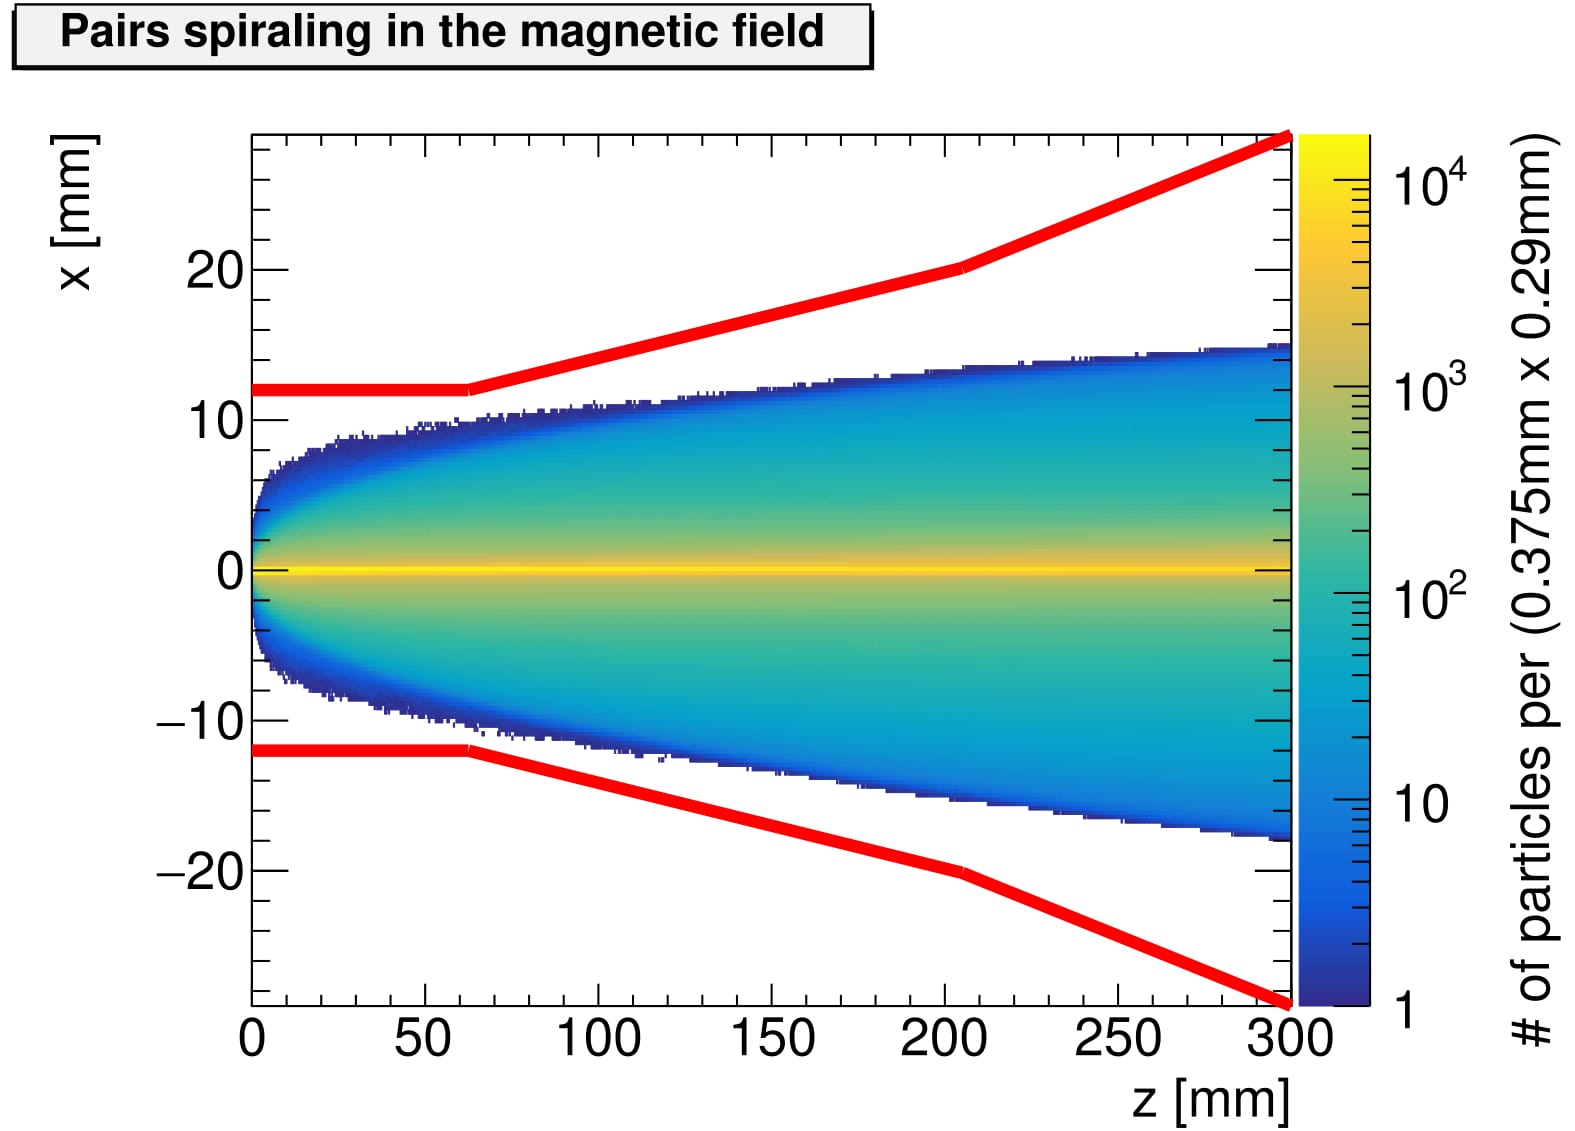
\includegraphics[width=\textwidth]{figures/Helix_tracks_xz_100bunches_250GeV_5T_DanielJeans-1.jpg}
\caption{\textit{ILC250 set (TDR)}}
\end{subfigure}
\hspace*{0.08cm}
\begin{subfigure}[t]{0.49\textwidth}
\centering
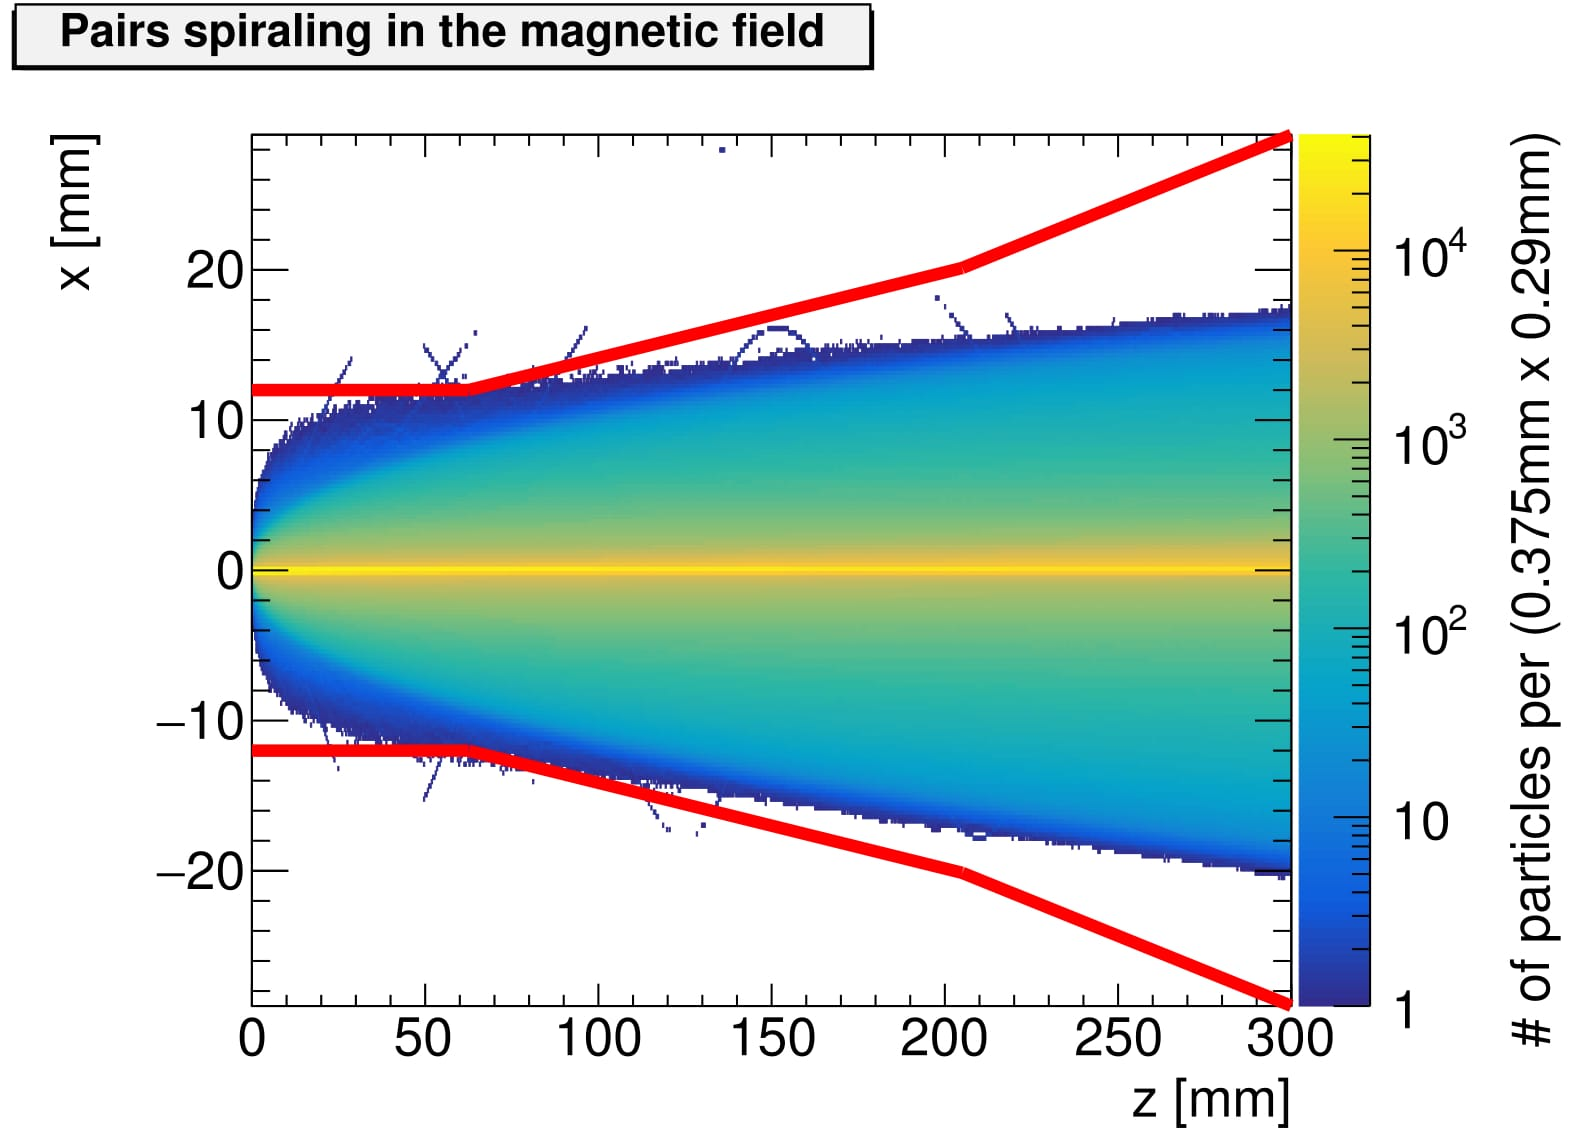
\includegraphics[width=\textwidth]{figures/Helix_tracks_xz_80bunches_250GeV_5T_Reduced_Emittance_x-1.jpg}
\caption{\textit{ILC250 set (A)}}
\end{subfigure}
\\
\begin{subfigure}[t]{0.49\textwidth}
\centering
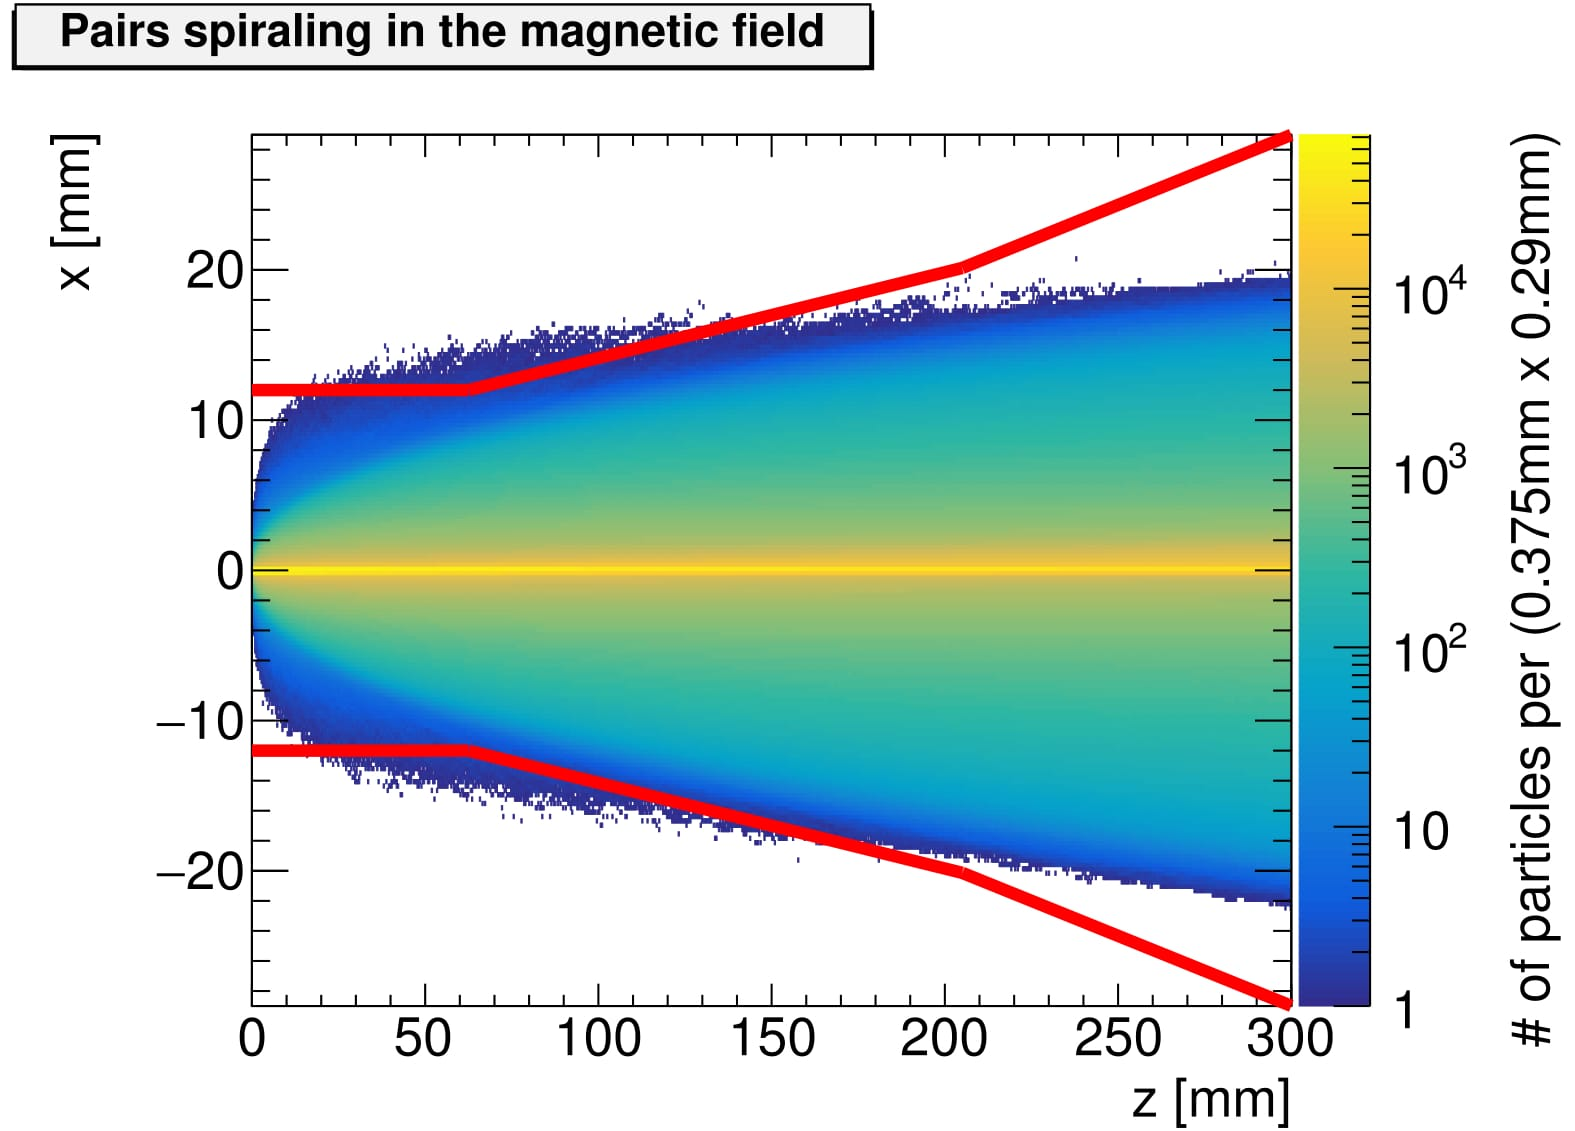
\includegraphics[width=\textwidth]{figures/Helix_tracks_xz_50bunches_250GeV_5T_Reduced_Emittance_x_Reduced_Beta_x-1.jpg}
\caption{\textit{ILC250 set (B)}}
\end{subfigure}
\hspace*{0.08cm}
\begin{subfigure}[t]{0.49\textwidth}
\centering
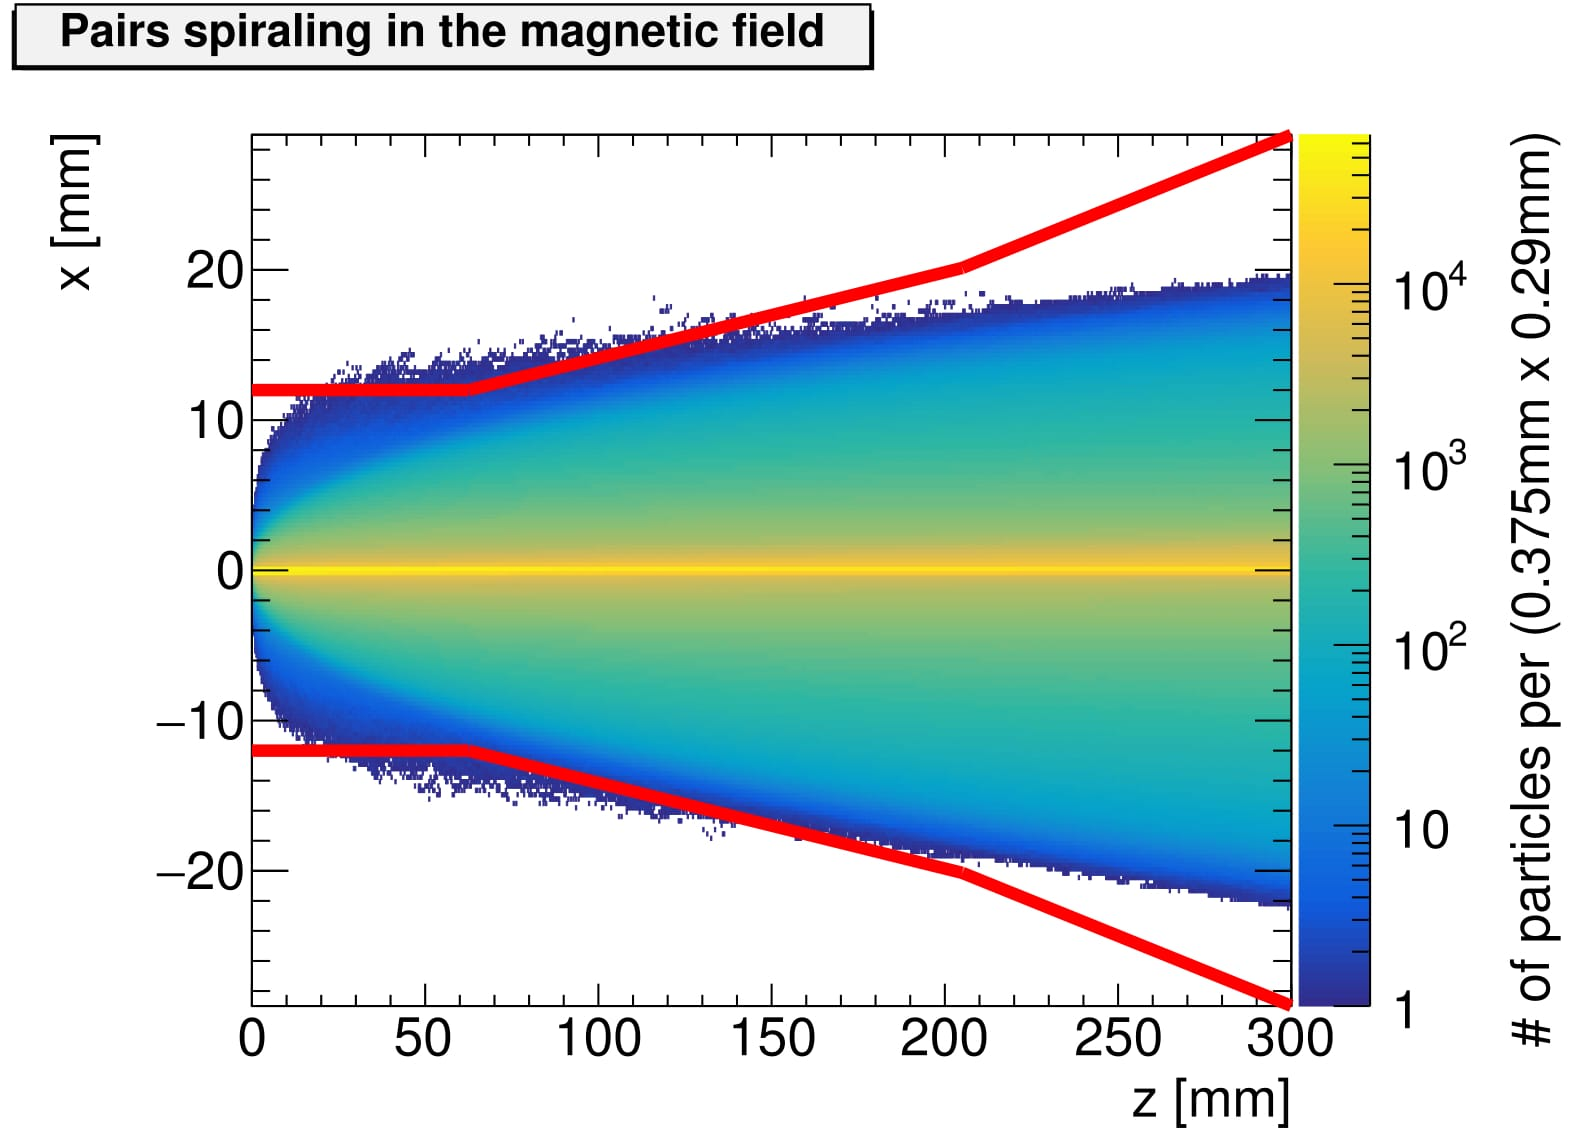
\includegraphics[width=\textwidth]{figures/Helix_tracks_xz_50bunches_250GeV_5T_Reduced_Emittance_x_Reduced_Beta_x_Increased_Beta_y-1.jpg}
\caption{\textit{ILC250 set (C)}}
\end{subfigure}
\caption{\textit{Pair background density for the different ILC250 beam parameter sets. Although the pairs are deflected in the SiD solenoid field, the high-p\textsubscript{T} pairs reach past the beam pipe towards the inner layers of the detector. The beam pipe is represented by the red solid lines.}}
\label{fig:Envelopes}
\end{figure}


\begin{figure}
\centering
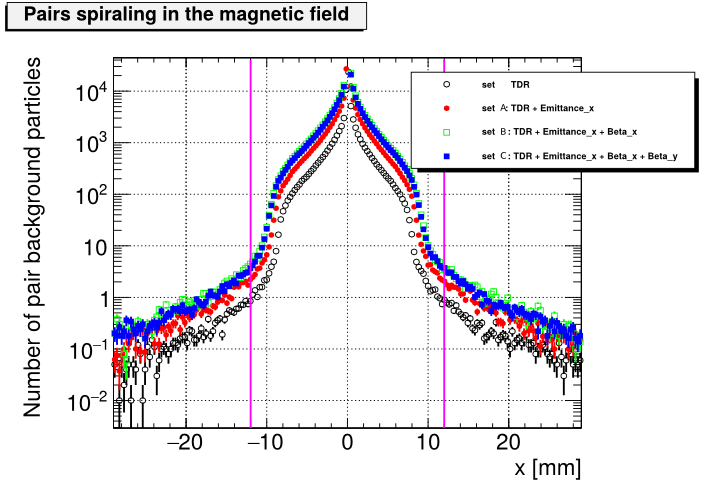
\includegraphics[width=\textwidth]{figures/HelixEnvelope_Projection_Comparison_250GeV_parametersets_NEWSETNAMES.png}
\caption{\textit{Projection of the pair background density shown in Figure~\ref{fig:Envelopes} along the x direction.
The projection is done for z $=$ \SI{62}{\milli\meter}, the z position of the first beam pipe kink.
At that position, the background envelopes are the largest compared to the beam pipe radius.
The beam pipe is indicated by the pink solid lines.}}
\label{fig:Projection_Envelopes}
\end{figure}

\iffalse
    The projection of the helix tracks from the pair background particles of one bunch crossing are shown in the xz- and yz-plane in Figures a) and c).
    The color scales shows how many particle tracks are in the single bins of these plots.
    To get a better grasp, Figures b) and d) show the envelopes outlining certain fractions of helix tracks.
    Therefore, the blue line represents the envelope of 99\% of all pair tracks.
    In all subfigures, the thin red lines represent the beam pipe.
    The helix tracks were calculated for a homogeneous magnetic field of \unit{5}\,{T}.
\fi